\documentclass[11pt]{article}
\usepackage[letterpaper,margin=0.75in,headheight=15pt]{geometry}
\usepackage[T1]{fontenc}
\usepackage{lmodern,booktabs,longtable,array,graphicx,tikz,xcolor,hyperref,fancyhdr}
\usetikzlibrary{arrows.meta}
\definecolor{navy}{HTML}{16374A}
\definecolor{pale}{HTML}{F2F5F6}
\definecolor{amber}{HTML}{F2F5F6}
\definecolor{muted}{HTML}{576976}
\hypersetup{colorlinks=true,linkcolor=navy,urlcolor=navy,pdftitle={VCU Configuration Record},bookmarksopen=false}
\renewcommand{\familydefault}{\sfdefault}
\setlength{\parindent}{0pt}
\setlength{\parskip}{6pt}
\setlength{\emergencystretch}{3em}
\setcounter{tocdepth}{1}
\raggedbottom
\pagestyle{fancy}\fancyhf{}
\fancyhead[L]{\footnotesize\color{muted}TRIDENT / VCU}
\fancyhead[R]{\footnotesize\hyperref[overview]{Overview}\quad\hyperref[appendices]{Appendices}}
\renewcommand{\headrulewidth}{0pt}
\renewcommand{\footrulewidth}{0pt}
\newcommand{\notebox}[1]{\par\noindent\colorbox{pale}{\parbox{\dimexpr\linewidth-2\fboxsep\relax}{#1}}\par}

\fancyfoot[L]{\footnotesize\color{muted}VCU-REV9-DRAFT-007 / Draft}
\fancyfoot[R]{\footnotesize\thepage}
\begin{document}
{\color{navy}\LARGE\bfseries VCU configuration record}\par
\refstepcounter{section}\label{overview}\addcontentsline{toc}{section}{\protect\numberline{1}Configuration overview}
{\color{muted}Flow-loop setup, instruments and supporting evidence}\par\vspace{8pt}
\textbf{Configuration:} VCU-REV9-DRAFT-007\par
\textbf{Effective date:} 2026-10-16\par
\textbf{Status:} Draft\par
\textbf{Basis:} Rev9 CAD candidate. The installed configuration has not yet been verified.\par
\vspace{8pt}
\begin{center}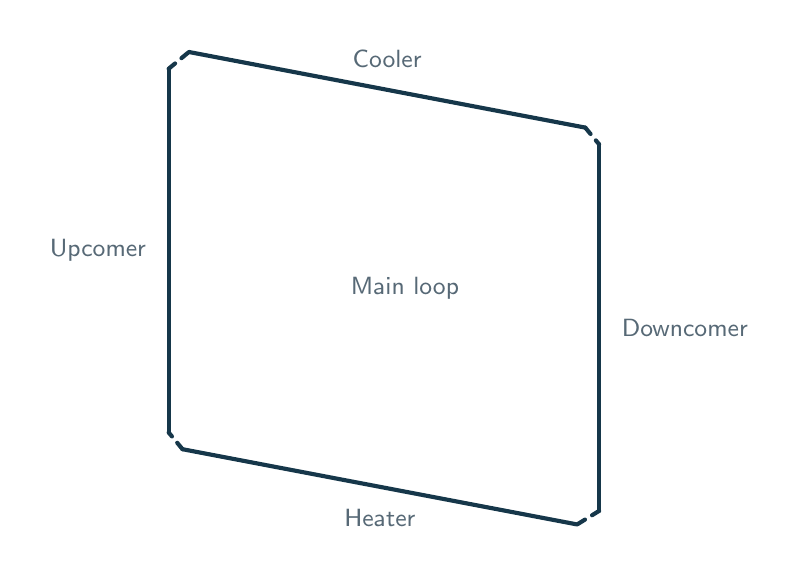
\begin{tikzpicture}[line cap=round,line join=round]
\draw[navy,line width=1.5pt] (0.0000,1.1681) -- (0.0000,5.7873);
\draw[navy,line width=1.5pt,dashed] (0.0000,5.7873) -- (0.2571,6.0000);
\draw[navy,line width=1.5pt] (0.2571,6.0000) -- (5.2908,5.0398);
\draw[navy,line width=1.5pt,dashed] (5.2908,5.0398) -- (5.4668,4.8271);
\draw[navy,line width=1.5pt] (5.4668,4.8271) -- (5.4668,0.1720);
\draw[navy,line width=1.5pt,dashed] (5.4668,0.1720) -- (5.1872,0.0000);
\draw[navy,line width=1.5pt] (5.1872,0.0000) -- (0.1760,0.9554);
\draw[navy,line width=1.5pt,dashed] (0.1760,0.9554) -- (0.0000,1.1681);
\node[font=\small,text=muted,left,inner sep=8pt] at (0.0000,3.4777) {Upcomer};
\node[font=\small,text=muted,above,inner sep=8pt] at (2.7740,5.5199) {Cooler};
\node[font=\small,text=muted,right,inner sep=8pt] at (5.4668,2.4995) {Downcomer};
\node[font=\small,text=muted,below,inner sep=8pt] at (2.6816,0.4777) {Heater};
\node[text=muted,font=\small] at (3,3) {Main loop};
\end{tikzpicture}\par{\footnotesize\color{muted}CAD overview. Dashed corners are schematic.}\end{center}
\vspace{4pt}{\large\bfseries Read the configuration}\par
\hyperref[geometry-main]{Geometry}\quad / \quad\hyperref[insulation-main]{Insulation}\quad / \quad\hyperref[instruments-main]{Instruments}\par
\hyperref[thermal-main]{Heating and cooling}\quad / \quad\hyperref[materials-main]{Materials and fluids}\par
\hyperref[uncertainty-main]{Uncertainty and limitations}\par
\vspace{8pt}\textbf{Adding information?} Open \texttt{VCU\_inputs.xlsx} and start with one Form tab. \hyperref[administration]{Contributor instructions} and \hyperref[appendices]{supporting records} are in the appendices.\par
{\footnotesize\color{muted}Unknown values remain open. This draft records available evidence; it is not a released facility description.}\par
\clearpage\section{Geometry}\label{geometry-main}
Axis-end dimensions and the recorded jacket envelope. Bore and insulation measurements remain open.
\begin{center}\resizebox{0.93\textwidth}{!}{%
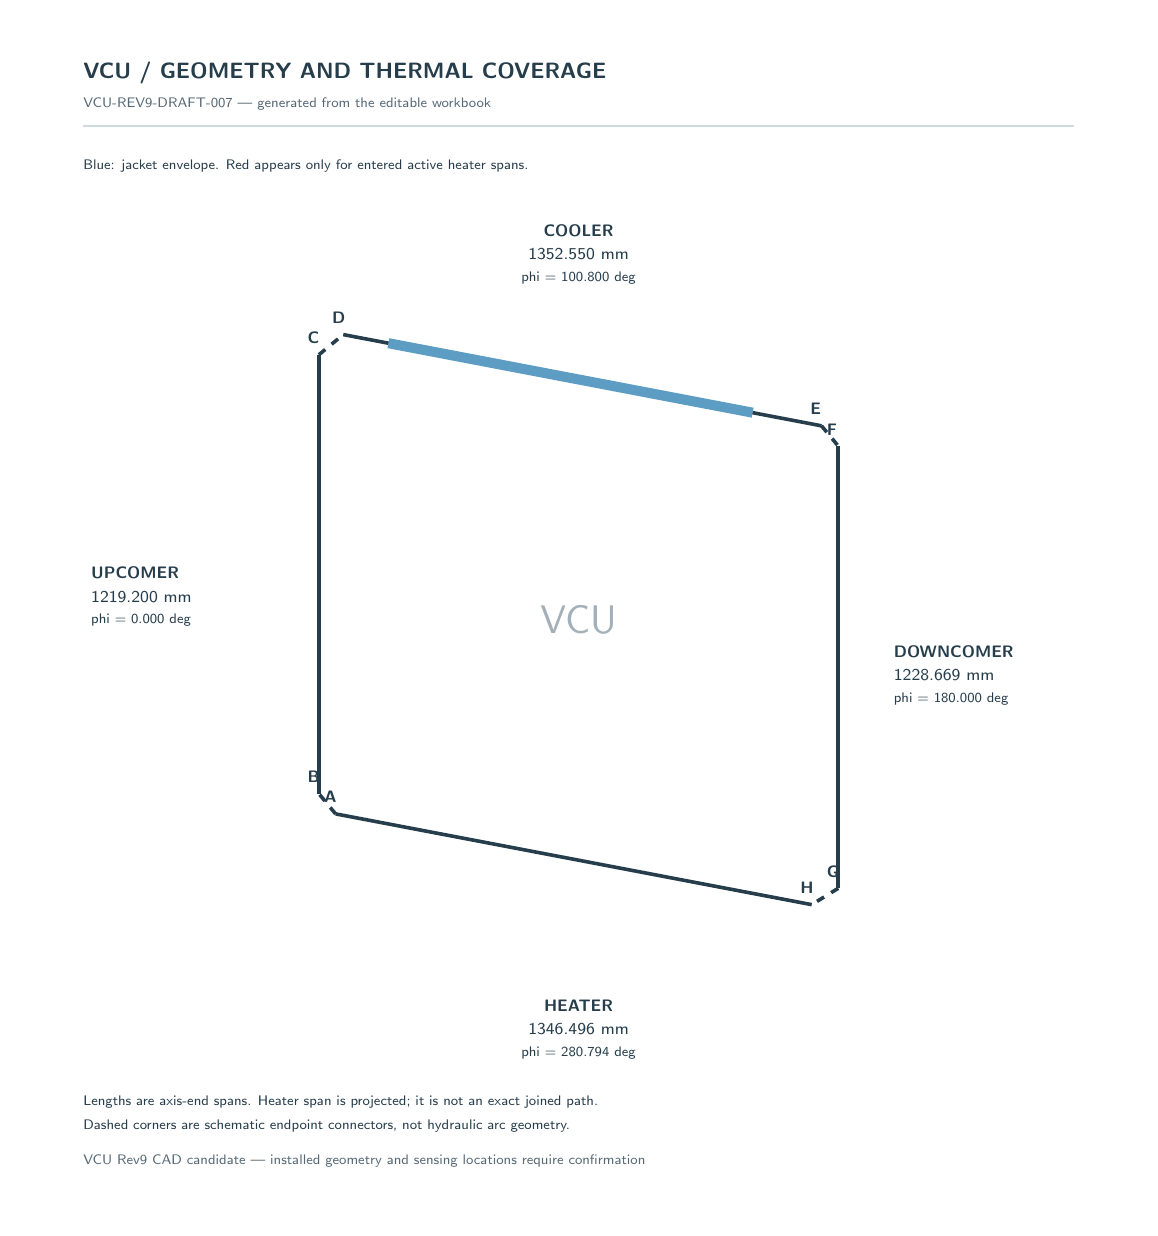
\begin{tikzpicture}[x=0.01cm,y=-0.01cm]
\path[use as bounding box] (0,0) rectangle (1400,1500);
\definecolor{c263D4B}{HTML}{263D4B}
\definecolor{c576976}{HTML}{576976}
\definecolor{c5D9DC3}{HTML}{5D9DC3}
\definecolor{cA3B0B9}{HTML}{A3B0B9}
\definecolor{cCFD9DF}{HTML}{CFD9DF}
\node[anchor=base west,inner sep=0pt,text=c263D4B,font=\sffamily\fontsize{8.40}{10.20}\selectfont\bfseries] at (70.000,65.000) {VCU / GEOMETRY AND THERMAL COVERAGE};
\node[anchor=base west,inner sep=0pt,text=c576976,font=\sffamily\fontsize{4.76}{5.78}\selectfont] at (70.000,102.000) {VCU-REV9-DRAFT-007 | generated from the editable workbook};
\draw[draw=cCFD9DF,line width=0.520pt] (70.000,125.000) -- (1330.000,125.000);
\draw[draw=c263D4B,line width=1.300pt] (370.000,973.358) -- (370.000,415.678);
\draw[draw=c263D4B,line width=1.300pt,dashed] (370.000,415.678) -- (401.040,390.000);
\draw[draw=c263D4B,line width=1.300pt] (401.040,390.000) -- (1008.757,505.928);
\draw[draw=c263D4B,line width=1.300pt,dashed] (1008.757,505.928) -- (1030.000,531.607);
\draw[draw=c263D4B,line width=1.300pt] (1030.000,531.607) -- (1030.000,1093.617);
\draw[draw=c263D4B,line width=1.300pt,dashed] (1030.000,1093.617) -- (996.253,1114.378);
\draw[draw=c263D4B,line width=1.300pt] (996.253,1114.378) -- (391.243,999.036);
\draw[draw=c263D4B,line width=1.300pt,dashed] (391.243,999.036) -- (370.000,973.358);
\draw[draw=c5D9DC3,line width=3.640pt] (458.355,400.933) -- (921.276,489.240);
\node[anchor=base west,inner sep=0pt,text=c263D4B,font=\sffamily\fontsize{5.60}{6.80}\selectfont\bfseries] at (355.000,959.358) {B};
\node[anchor=base west,inner sep=0pt,text=c263D4B,font=\sffamily\fontsize{5.60}{6.80}\selectfont\bfseries] at (355.000,401.678) {C};
\node[anchor=base west,inner sep=0pt,text=c263D4B,font=\sffamily\fontsize{5.60}{6.80}\selectfont\bfseries] at (386.040,376.000) {D};
\node[anchor=base west,inner sep=0pt,text=c263D4B,font=\sffamily\fontsize{5.60}{6.80}\selectfont\bfseries] at (993.757,491.928) {E};
\node[anchor=base west,inner sep=0pt,text=c263D4B,font=\sffamily\fontsize{5.60}{6.80}\selectfont\bfseries] at (1015.000,517.607) {F};
\node[anchor=base west,inner sep=0pt,text=c263D4B,font=\sffamily\fontsize{5.60}{6.80}\selectfont\bfseries] at (1015.000,1079.617) {G};
\node[anchor=base west,inner sep=0pt,text=c263D4B,font=\sffamily\fontsize{5.60}{6.80}\selectfont\bfseries] at (981.253,1100.378) {H};
\node[anchor=base west,inner sep=0pt,text=c263D4B,font=\sffamily\fontsize{5.60}{6.80}\selectfont\bfseries] at (376.243,985.036) {A};
\node[anchor=base,inner sep=0pt,text=cA3B0B9,font=\sffamily\fontsize{15.12}{18.36}\selectfont] at (700.000,770.000) {VCU};
\node[anchor=base west,inner sep=0pt,text=c263D4B,font=\sffamily\fontsize{6.16}{7.48}\selectfont\bfseries] at (80.000,700.000) {UPCOMER};
\node[anchor=base west,inner sep=0pt,text=c263D4B,font=\sffamily\fontsize{5.60}{6.80}\selectfont] at (80.000,730.000) {1219.200 mm};
\node[anchor=base west,inner sep=0pt,text=c263D4B,font=\sffamily\fontsize{4.76}{5.78}\selectfont] at (80.000,757.000) {phi = 0.000 deg};
\node[anchor=base,inner sep=0pt,text=c263D4B,font=\sffamily\fontsize{6.16}{7.48}\selectfont\bfseries] at (700.000,265.000) {COOLER};
\node[anchor=base,inner sep=0pt,text=c263D4B,font=\sffamily\fontsize{5.60}{6.80}\selectfont] at (700.000,295.000) {1352.550 mm};
\node[anchor=base,inner sep=0pt,text=c263D4B,font=\sffamily\fontsize{4.76}{5.78}\selectfont] at (700.000,322.000) {phi = 100.800 deg};
\node[anchor=base west,inner sep=0pt,text=c263D4B,font=\sffamily\fontsize{6.16}{7.48}\selectfont\bfseries] at (1100.000,800.000) {DOWNCOMER};
\node[anchor=base west,inner sep=0pt,text=c263D4B,font=\sffamily\fontsize{5.60}{6.80}\selectfont] at (1100.000,830.000) {1228.669 mm};
\node[anchor=base west,inner sep=0pt,text=c263D4B,font=\sffamily\fontsize{4.76}{5.78}\selectfont] at (1100.000,857.000) {phi = 180.000 deg};
\node[anchor=base,inner sep=0pt,text=c263D4B,font=\sffamily\fontsize{6.16}{7.48}\selectfont\bfseries] at (700.000,1250.000) {HEATER};
\node[anchor=base,inner sep=0pt,text=c263D4B,font=\sffamily\fontsize{5.60}{6.80}\selectfont] at (700.000,1280.000) {1346.496 mm};
\node[anchor=base,inner sep=0pt,text=c263D4B,font=\sffamily\fontsize{4.76}{5.78}\selectfont] at (700.000,1307.000) {phi = 280.794 deg};
\node[anchor=base west,inner sep=0pt,text=c263D4B,font=\sffamily\fontsize{5.04}{6.12}\selectfont] at (70.000,180.000) {Blue: jacket envelope. Red appears only for entered active heater spans.};
\node[anchor=base west,inner sep=0pt,text=c263D4B,font=\sffamily\fontsize{4.76}{5.78}\selectfont] at (70.000,1370.000) {Lengths are axis-end spans. Heater span is projected; it is not an exact joined path.};
\node[anchor=base west,inner sep=0pt,text=c263D4B,font=\sffamily\fontsize{4.76}{5.78}\selectfont] at (70.000,1400.000) {Dashed corners are schematic endpoint connectors, not hydraulic arc geometry.};
\node[anchor=base west,inner sep=0pt,text=c576976,font=\sffamily\fontsize{4.48}{5.44}\selectfont] at (70.000,1445.000) {VCU Rev9 CAD candidate | installed geometry and sensing locations require confirmation};
\end{tikzpicture}
}\end{center}
{\small Details: \hyperref[geometry-detail]{coordinate conventions and CAD qualifications}; \hyperref[baseline-tables]{dimension tables}.}\par
\clearpage\section{Insulation}\label{insulation-main}
Use the workbook\textquotesingle s \textbf{Insulation regions} tab. Every coverage dropdown describes the whole named region.
\begin{center}\resizebox{0.93\textwidth}{!}{%
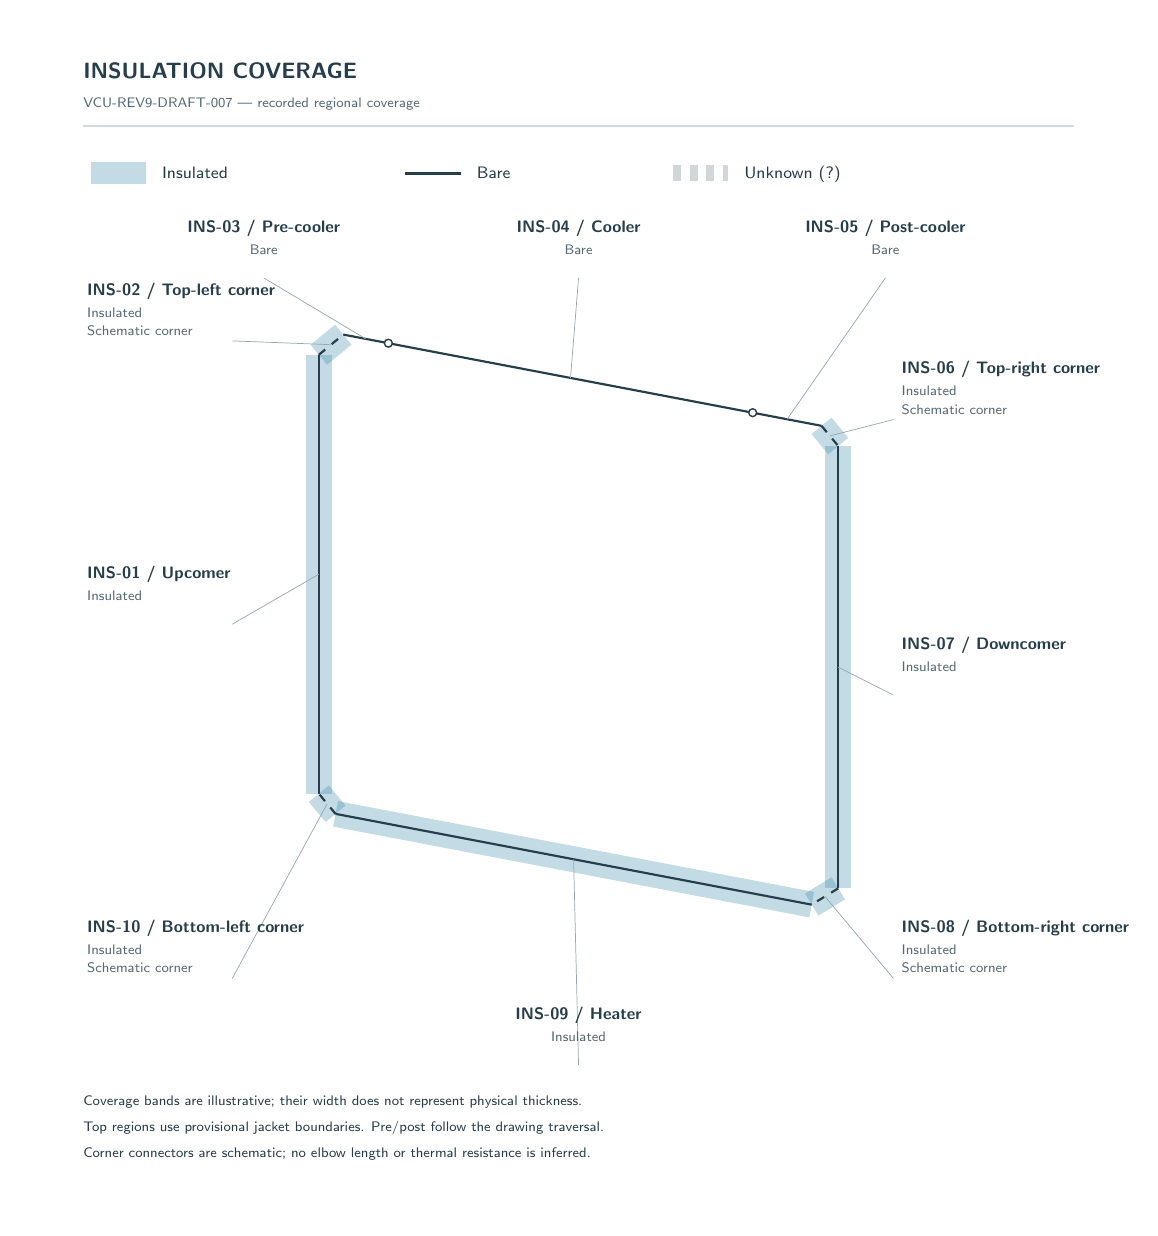
\begin{tikzpicture}[x=0.01cm,y=-0.01cm]
\path[use as bounding box] (0,0) rectangle (1400,1500);
\definecolor{c263D4B}{HTML}{263D4B}
\definecolor{c287FA3}{HTML}{287FA3}
\definecolor{c576976}{HTML}{576976}
\definecolor{c7B8992}{HTML}{7B8992}
\definecolor{c98A7B1}{HTML}{98A7B1}
\definecolor{cCFD9DF}{HTML}{CFD9DF}
\node[anchor=base west,inner sep=0pt,text=c263D4B,font=\sffamily\fontsize{8.40}{10.20}\selectfont\bfseries] at (70.000,65.000) {INSULATION COVERAGE};
\node[anchor=base west,inner sep=0pt,text=c576976,font=\sffamily\fontsize{4.76}{5.78}\selectfont] at (70.000,102.000) {VCU-REV9-DRAFT-007 | recorded regional coverage};
\draw[draw=cCFD9DF,line width=0.520pt] (70.000,125.000) -- (1330.000,125.000);
\draw[draw=c287FA3,line width=7.800pt,draw opacity=0.28] (80.000,185.000) -- (150.000,185.000);
\node[anchor=base west,inner sep=0pt,text=c263D4B,font=\sffamily\fontsize{6.44}{7.82}\selectfont] at (170.000,192.000) {Insulated};
\draw[draw=c263D4B,line width=1.040pt] (480.000,185.000) -- (550.000,185.000);
\node[anchor=base west,inner sep=0pt,text=c263D4B,font=\sffamily\fontsize{6.44}{7.82}\selectfont] at (570.000,192.000) {Bare};
\draw[draw=c7B8992,line width=5.720pt,dashed,draw opacity=0.35] (820.000,185.000) -- (890.000,185.000);
\node[anchor=base west,inner sep=0pt,text=c263D4B,font=\sffamily\fontsize{6.44}{7.82}\selectfont] at (910.000,192.000) {Unknown (?)};
\draw[draw=c287FA3,line width=9.360pt,draw opacity=0.28] (370.000,973.358) -- (370.000,415.678);
\draw[draw=c287FA3,line width=9.360pt,draw opacity=0.28] (370.000,415.678) -- (401.040,390.000);
\draw[draw=c287FA3,line width=9.360pt,draw opacity=0.28] (1008.757,505.928) -- (1030.000,531.607);
\draw[draw=c287FA3,line width=9.360pt,draw opacity=0.28] (1030.000,531.607) -- (1030.000,1093.617);
\draw[draw=c287FA3,line width=9.360pt,draw opacity=0.28] (1030.000,1093.617) -- (996.253,1114.378);
\draw[draw=c287FA3,line width=9.360pt,draw opacity=0.28] (996.253,1114.378) -- (391.243,999.036);
\draw[draw=c287FA3,line width=9.360pt,draw opacity=0.28] (391.243,999.036) -- (370.000,973.358);
\draw[draw=c263D4B,line width=0.780pt] (370.000,973.358) -- (370.000,415.678);
\draw[draw=c263D4B,line width=0.780pt,dashed] (370.000,415.678) -- (401.040,390.000);
\draw[draw=c263D4B,line width=0.780pt] (401.040,390.000) -- (1008.757,505.928);
\draw[draw=c263D4B,line width=0.780pt,dashed] (1008.757,505.928) -- (1030.000,531.607);
\draw[draw=c263D4B,line width=0.780pt] (1030.000,531.607) -- (1030.000,1093.617);
\draw[draw=c263D4B,line width=0.780pt,dashed] (1030.000,1093.617) -- (996.253,1114.378);
\draw[draw=c263D4B,line width=0.780pt] (996.253,1114.378) -- (391.243,999.036);
\draw[draw=c263D4B,line width=0.780pt,dashed] (391.243,999.036) -- (370.000,973.358);
\draw[draw=c98A7B1,line width=0.260pt] (370.000,694.518) -- (260.000,758.000);
\node[anchor=base west,inner sep=0pt,text=c263D4B,font=\sffamily\fontsize{5.60}{6.80}\selectfont\bfseries] at (75.000,700.000) {INS-01 / Upcomer};
\node[anchor=base west,inner sep=0pt,text=c576976,font=\sffamily\fontsize{5.32}{6.46}\selectfont] at (75.000,728.000) {Insulated};
\draw[draw=c98A7B1,line width=0.260pt] (385.520,402.839) -- (260.000,398.000);
\node[anchor=base west,inner sep=0pt,text=c263D4B,font=\sffamily\fontsize{5.60}{6.80}\selectfont\bfseries] at (75.000,340.000) {INS-02 / Top-left corner};
\node[anchor=base west,inner sep=0pt,text=c576976,font=\sffamily\fontsize{5.32}{6.46}\selectfont] at (75.000,368.000) {Insulated};
\node[anchor=base west,inner sep=0pt,text=c576976,font=\sffamily\fontsize{4.48}{5.44}\selectfont] at (75.000,391.000) {Schematic corner};
\draw[draw=c98A7B1,line width=0.260pt] (429.697,395.467) -- (300.000,318.000);
\node[anchor=base,inner sep=0pt,text=c263D4B,font=\sffamily\fontsize{5.60}{6.80}\selectfont\bfseries] at (300.000,260.000) {INS-03 / Pre-cooler};
\node[anchor=base,inner sep=0pt,text=c576976,font=\sffamily\fontsize{5.32}{6.46}\selectfont] at (300.000,288.000) {Bare};
\draw[draw=c98A7B1,line width=0.260pt] (689.815,445.087) -- (700.000,318.000);
\node[anchor=base,inner sep=0pt,text=c263D4B,font=\sffamily\fontsize{5.60}{6.80}\selectfont\bfseries] at (700.000,260.000) {INS-04 / Cooler};
\node[anchor=base,inner sep=0pt,text=c576976,font=\sffamily\fontsize{5.32}{6.46}\selectfont] at (700.000,288.000) {Bare};
\draw[draw=c98A7B1,line width=0.260pt] (965.016,497.584) -- (1090.000,318.000);
\node[anchor=base,inner sep=0pt,text=c263D4B,font=\sffamily\fontsize{5.60}{6.80}\selectfont\bfseries] at (1090.000,260.000) {INS-05 / Post-cooler};
\node[anchor=base,inner sep=0pt,text=c576976,font=\sffamily\fontsize{5.32}{6.46}\selectfont] at (1090.000,288.000) {Bare};
\draw[draw=c98A7B1,line width=0.260pt] (1019.379,518.767) -- (1100.000,498.000);
\node[anchor=base west,inner sep=0pt,text=c263D4B,font=\sffamily\fontsize{5.60}{6.80}\selectfont\bfseries] at (1110.000,440.000) {INS-06 / Top-right corner};
\node[anchor=base west,inner sep=0pt,text=c576976,font=\sffamily\fontsize{5.32}{6.46}\selectfont] at (1110.000,468.000) {Insulated};
\node[anchor=base west,inner sep=0pt,text=c576976,font=\sffamily\fontsize{4.48}{5.44}\selectfont] at (1110.000,491.000) {Schematic corner};
\draw[draw=c98A7B1,line width=0.260pt] (1030.000,812.612) -- (1100.000,848.000);
\node[anchor=base west,inner sep=0pt,text=c263D4B,font=\sffamily\fontsize{5.60}{6.80}\selectfont\bfseries] at (1110.000,790.000) {INS-07 / Downcomer};
\node[anchor=base west,inner sep=0pt,text=c576976,font=\sffamily\fontsize{5.32}{6.46}\selectfont] at (1110.000,818.000) {Insulated};
\draw[draw=c98A7B1,line width=0.260pt] (1013.127,1103.997) -- (1100.000,1208.000);
\node[anchor=base west,inner sep=0pt,text=c263D4B,font=\sffamily\fontsize{5.60}{6.80}\selectfont\bfseries] at (1110.000,1150.000) {INS-08 / Bottom-right corner};
\node[anchor=base west,inner sep=0pt,text=c576976,font=\sffamily\fontsize{5.32}{6.46}\selectfont] at (1110.000,1178.000) {Insulated};
\node[anchor=base west,inner sep=0pt,text=c576976,font=\sffamily\fontsize{4.48}{5.44}\selectfont] at (1110.000,1201.000) {Schematic corner};
\draw[draw=c98A7B1,line width=0.260pt] (693.748,1056.707) -- (700.000,1318.000);
\node[anchor=base,inner sep=0pt,text=c263D4B,font=\sffamily\fontsize{5.60}{6.80}\selectfont\bfseries] at (700.000,1260.000) {INS-09 / Heater};
\node[anchor=base,inner sep=0pt,text=c576976,font=\sffamily\fontsize{5.32}{6.46}\selectfont] at (700.000,1288.000) {Insulated};
\draw[draw=c98A7B1,line width=0.260pt] (380.621,986.197) -- (260.000,1208.000);
\node[anchor=base west,inner sep=0pt,text=c263D4B,font=\sffamily\fontsize{5.60}{6.80}\selectfont\bfseries] at (75.000,1150.000) {INS-10 / Bottom-left corner};
\node[anchor=base west,inner sep=0pt,text=c576976,font=\sffamily\fontsize{5.32}{6.46}\selectfont] at (75.000,1178.000) {Insulated};
\node[anchor=base west,inner sep=0pt,text=c576976,font=\sffamily\fontsize{4.48}{5.44}\selectfont] at (75.000,1201.000) {Schematic corner};
\draw[fill=white,draw=c263D4B,line width=0.5pt] (458.355,400.933) circle (5);
\draw[fill=white,draw=c263D4B,line width=0.5pt] (921.276,489.240) circle (5);
\node[anchor=base west,inner sep=0pt,text=c263D4B,font=\sffamily\fontsize{5.04}{6.12}\selectfont] at (70.000,1370.000) {Coverage bands are illustrative; their width does not represent physical thickness.};
\node[anchor=base west,inner sep=0pt,text=c263D4B,font=\sffamily\fontsize{5.04}{6.12}\selectfont] at (70.000,1403.000) {Top regions use provisional jacket boundaries. Pre/post follow the drawing traversal.};
\node[anchor=base west,inner sep=0pt,text=c263D4B,font=\sffamily\fontsize{5.04}{6.12}\selectfont] at (70.000,1436.000) {Corner connectors are schematic; no elbow length or thermal resistance is inferred.};
\end{tikzpicture}
}\end{center}
{\small Details: \hyperref[insulation-detail]{materials, thickness and evidence by region}. No resistance factors or boundary conditions are calculated.}\par
\clearpage\section{Instruments}\label{instruments-main}
Geometric sensor references on the main loop. Working native-channel bindings are documented separately; installed junctions and calibration still require evidence.
\begin{center}\resizebox{0.93\textwidth}{!}{%
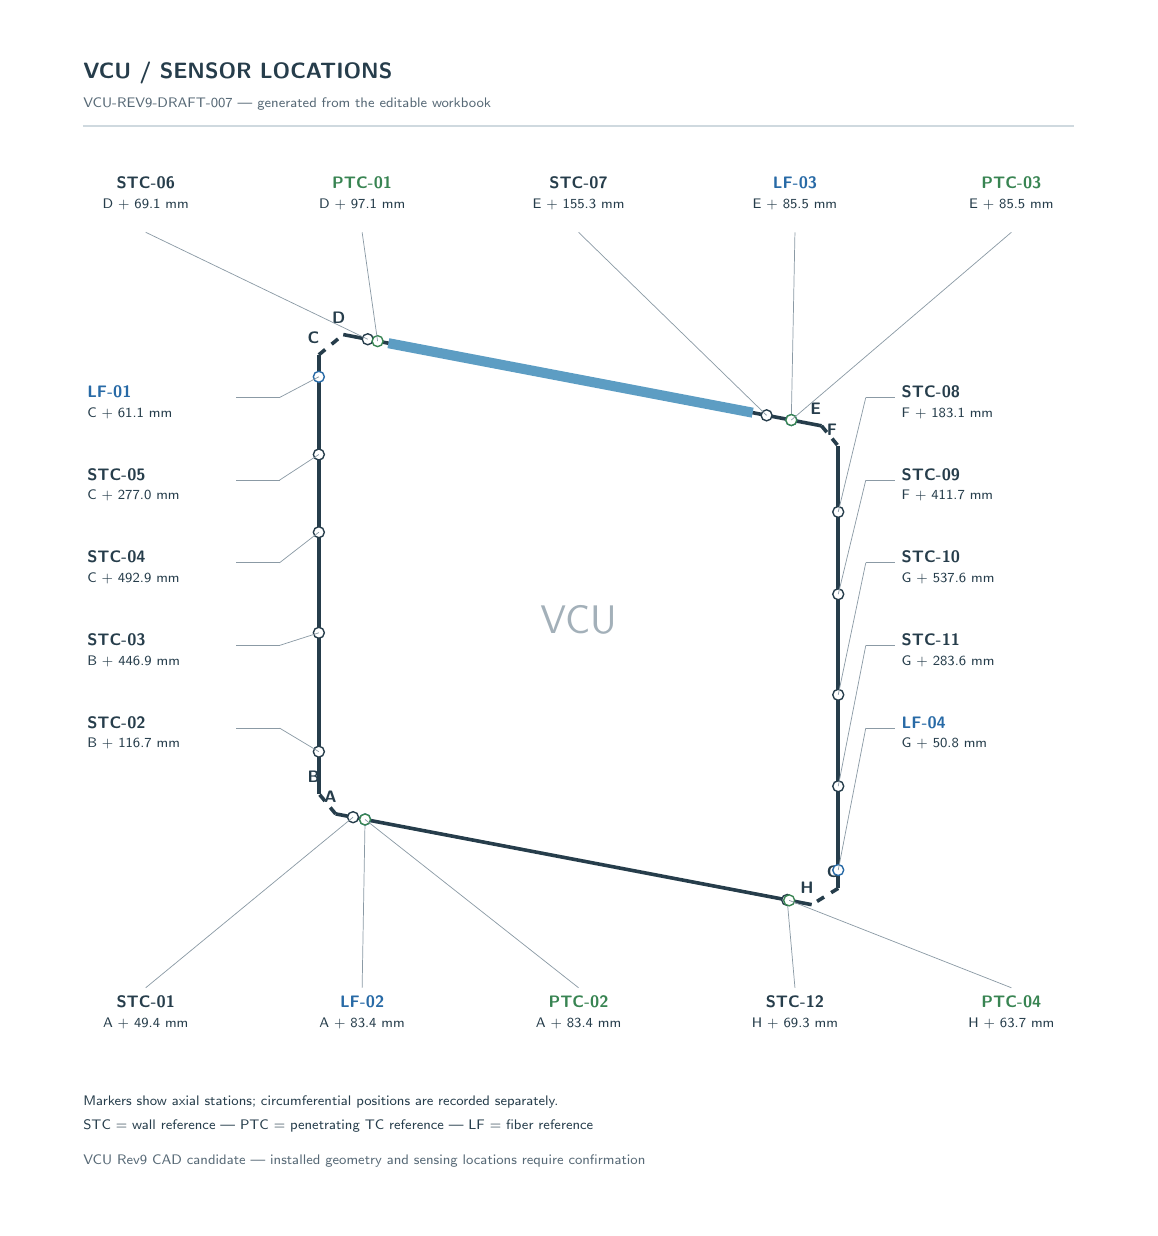
\begin{tikzpicture}[x=0.01cm,y=-0.01cm]
\path[use as bounding box] (0,0) rectangle (1400,1500);
\definecolor{c263D4B}{HTML}{263D4B}
\definecolor{c286AA6}{HTML}{286AA6}
\definecolor{c388452}{HTML}{388452}
\definecolor{c576976}{HTML}{576976}
\definecolor{c5D9DC3}{HTML}{5D9DC3}
\definecolor{c8B9AA5}{HTML}{8B9AA5}
\definecolor{cA3B0B9}{HTML}{A3B0B9}
\definecolor{cCFD9DF}{HTML}{CFD9DF}
\node[anchor=base west,inner sep=0pt,text=c263D4B,font=\sffamily\fontsize{8.40}{10.20}\selectfont\bfseries] at (70.000,65.000) {VCU / SENSOR LOCATIONS};
\node[anchor=base west,inner sep=0pt,text=c576976,font=\sffamily\fontsize{4.76}{5.78}\selectfont] at (70.000,102.000) {VCU-REV9-DRAFT-007 | generated from the editable workbook};
\draw[draw=cCFD9DF,line width=0.520pt] (70.000,125.000) -- (1330.000,125.000);
\draw[draw=c263D4B,line width=1.300pt] (370.000,973.358) -- (370.000,415.678);
\draw[draw=c263D4B,line width=1.300pt,dashed] (370.000,415.678) -- (401.040,390.000);
\draw[draw=c263D4B,line width=1.300pt] (401.040,390.000) -- (1008.757,505.928);
\draw[draw=c263D4B,line width=1.300pt,dashed] (1008.757,505.928) -- (1030.000,531.607);
\draw[draw=c263D4B,line width=1.300pt] (1030.000,531.607) -- (1030.000,1093.617);
\draw[draw=c263D4B,line width=1.300pt,dashed] (1030.000,1093.617) -- (996.253,1114.378);
\draw[draw=c263D4B,line width=1.300pt] (996.253,1114.378) -- (391.243,999.036);
\draw[draw=c263D4B,line width=1.300pt,dashed] (391.243,999.036) -- (370.000,973.358);
\draw[draw=c5D9DC3,line width=3.640pt] (458.355,400.933) -- (921.276,489.240);
\node[anchor=base west,inner sep=0pt,text=c263D4B,font=\sffamily\fontsize{5.60}{6.80}\selectfont\bfseries] at (355.000,959.358) {B};
\node[anchor=base west,inner sep=0pt,text=c263D4B,font=\sffamily\fontsize{5.60}{6.80}\selectfont\bfseries] at (355.000,401.678) {C};
\node[anchor=base west,inner sep=0pt,text=c263D4B,font=\sffamily\fontsize{5.60}{6.80}\selectfont\bfseries] at (386.040,376.000) {D};
\node[anchor=base west,inner sep=0pt,text=c263D4B,font=\sffamily\fontsize{5.60}{6.80}\selectfont\bfseries] at (993.757,491.928) {E};
\node[anchor=base west,inner sep=0pt,text=c263D4B,font=\sffamily\fontsize{5.60}{6.80}\selectfont\bfseries] at (1015.000,517.607) {F};
\node[anchor=base west,inner sep=0pt,text=c263D4B,font=\sffamily\fontsize{5.60}{6.80}\selectfont\bfseries] at (1015.000,1079.617) {G};
\node[anchor=base west,inner sep=0pt,text=c263D4B,font=\sffamily\fontsize{5.60}{6.80}\selectfont\bfseries] at (981.253,1100.378) {H};
\node[anchor=base west,inner sep=0pt,text=c263D4B,font=\sffamily\fontsize{5.60}{6.80}\selectfont\bfseries] at (376.243,985.036) {A};
\node[anchor=base,inner sep=0pt,text=cA3B0B9,font=\sffamily\fontsize{15.12}{18.36}\selectfont] at (700.000,770.000) {VCU};
\draw[fill=white,draw=c286AA6,line width=0.5pt] (370.000,443.633) circle (7);
\draw[draw=c8B9AA5,line width=0.260pt] (370.000,443.633) -- (320.000,470.000);
\draw[draw=c8B9AA5,line width=0.260pt] (320.000,470.000) -- (265.000,470.000);
\node[anchor=base west,inner sep=0pt,text=c286AA6,font=\sffamily\fontsize{5.60}{6.80}\selectfont\bfseries] at (75.000,470.000) {LF-01};
\node[anchor=base west,inner sep=0pt,text=c263D4B,font=\sffamily\fontsize{4.48}{5.44}\selectfont] at (75.000,495.000) {C + 61.1 mm};
\draw[fill=white,draw=c263D4B,line width=0.5pt] (370.000,542.388) circle (7);
\draw[draw=c8B9AA5,line width=0.260pt] (370.000,542.388) -- (320.000,575.000);
\draw[draw=c8B9AA5,line width=0.260pt] (320.000,575.000) -- (265.000,575.000);
\node[anchor=base west,inner sep=0pt,text=c263D4B,font=\sffamily\fontsize{5.60}{6.80}\selectfont\bfseries] at (75.000,575.000) {STC-05};
\node[anchor=base west,inner sep=0pt,text=c263D4B,font=\sffamily\fontsize{4.48}{5.44}\selectfont] at (75.000,600.000) {C + 277.0 mm};
\draw[fill=white,draw=c263D4B,line width=0.5pt] (370.000,641.144) circle (7);
\draw[draw=c8B9AA5,line width=0.260pt] (370.000,641.144) -- (320.000,680.000);
\draw[draw=c8B9AA5,line width=0.260pt] (320.000,680.000) -- (265.000,680.000);
\node[anchor=base west,inner sep=0pt,text=c263D4B,font=\sffamily\fontsize{5.60}{6.80}\selectfont\bfseries] at (75.000,680.000) {STC-04};
\node[anchor=base west,inner sep=0pt,text=c263D4B,font=\sffamily\fontsize{4.48}{5.44}\selectfont] at (75.000,705.000) {C + 492.9 mm};
\draw[fill=white,draw=c263D4B,line width=0.5pt] (370.000,768.946) circle (7);
\draw[draw=c8B9AA5,line width=0.260pt] (370.000,768.946) -- (320.000,785.000);
\draw[draw=c8B9AA5,line width=0.260pt] (320.000,785.000) -- (265.000,785.000);
\node[anchor=base west,inner sep=0pt,text=c263D4B,font=\sffamily\fontsize{5.60}{6.80}\selectfont\bfseries] at (75.000,785.000) {STC-03};
\node[anchor=base west,inner sep=0pt,text=c263D4B,font=\sffamily\fontsize{4.48}{5.44}\selectfont] at (75.000,810.000) {B + 446.9 mm};
\draw[fill=white,draw=c263D4B,line width=0.5pt] (370.000,919.984) circle (7);
\draw[draw=c8B9AA5,line width=0.260pt] (370.000,919.984) -- (320.000,890.000);
\draw[draw=c8B9AA5,line width=0.260pt] (320.000,890.000) -- (265.000,890.000);
\node[anchor=base west,inner sep=0pt,text=c263D4B,font=\sffamily\fontsize{5.60}{6.80}\selectfont\bfseries] at (75.000,890.000) {STC-02};
\node[anchor=base west,inner sep=0pt,text=c263D4B,font=\sffamily\fontsize{4.48}{5.44}\selectfont] at (75.000,915.000) {B + 116.7 mm};
\draw[fill=white,draw=c263D4B,line width=0.5pt] (432.106,395.926) circle (7);
\draw[draw=c8B9AA5,line width=0.260pt] (432.106,395.926) -- (150.000,260.000);
\node[anchor=base,inner sep=0pt,text=c263D4B,font=\sffamily\fontsize{5.60}{6.80}\selectfont\bfseries] at (150.000,205.000) {STC-06};
\node[anchor=base,inner sep=0pt,text=c263D4B,font=\sffamily\fontsize{4.48}{5.44}\selectfont] at (150.000,230.000) {D + 69.1 mm};
\draw[fill=white,draw=c388452,line width=0.5pt] (444.659,398.321) circle (7);
\draw[draw=c8B9AA5,line width=0.260pt] (444.659,398.321) -- (425.000,260.000);
\node[anchor=base,inner sep=0pt,text=c388452,font=\sffamily\fontsize{5.60}{6.80}\selectfont\bfseries] at (425.000,205.000) {PTC-01};
\node[anchor=base,inner sep=0pt,text=c263D4B,font=\sffamily\fontsize{4.48}{5.44}\selectfont] at (425.000,230.000) {D + 97.1 mm};
\draw[fill=white,draw=c263D4B,line width=0.5pt] (938.965,492.615) circle (7);
\draw[draw=c8B9AA5,line width=0.260pt] (938.965,492.615) -- (700.000,260.000);
\node[anchor=base,inner sep=0pt,text=c263D4B,font=\sffamily\fontsize{5.60}{6.80}\selectfont\bfseries] at (700.000,205.000) {STC-07};
\node[anchor=base,inner sep=0pt,text=c263D4B,font=\sffamily\fontsize{4.48}{5.44}\selectfont] at (700.000,230.000) {E + 155.3 mm};
\draw[fill=white,draw=c286AA6,line width=0.5pt] (970.350,498.602) circle (7);
\draw[draw=c8B9AA5,line width=0.260pt] (970.350,498.602) -- (975.000,260.000);
\node[anchor=base,inner sep=0pt,text=c286AA6,font=\sffamily\fontsize{5.60}{6.80}\selectfont\bfseries] at (975.000,205.000) {LF-03};
\node[anchor=base,inner sep=0pt,text=c263D4B,font=\sffamily\fontsize{4.48}{5.44}\selectfont] at (975.000,230.000) {E + 85.5 mm};
\draw[fill=white,draw=c388452,line width=0.5pt] (970.350,498.602) circle (7);
\draw[draw=c8B9AA5,line width=0.260pt] (970.350,498.602) -- (1250.000,260.000);
\node[anchor=base,inner sep=0pt,text=c388452,font=\sffamily\fontsize{5.60}{6.80}\selectfont\bfseries] at (1250.000,205.000) {PTC-03};
\node[anchor=base,inner sep=0pt,text=c263D4B,font=\sffamily\fontsize{4.48}{5.44}\selectfont] at (1250.000,230.000) {E + 85.5 mm};
\draw[fill=white,draw=c263D4B,line width=0.5pt] (1030.000,615.361) circle (7);
\draw[draw=c8B9AA5,line width=0.260pt] (1030.000,615.361) -- (1065.000,470.000);
\draw[draw=c8B9AA5,line width=0.260pt] (1065.000,470.000) -- (1102.000,470.000);
\node[anchor=base west,inner sep=0pt,text=c263D4B,font=\sffamily\fontsize{5.60}{6.80}\selectfont\bfseries] at (1110.000,470.000) {STC-08};
\node[anchor=base west,inner sep=0pt,text=c263D4B,font=\sffamily\fontsize{4.48}{5.44}\selectfont] at (1110.000,495.000) {F + 183.1 mm};
\draw[fill=white,draw=c263D4B,line width=0.5pt] (1030.000,719.926) circle (7);
\draw[draw=c8B9AA5,line width=0.260pt] (1030.000,719.926) -- (1065.000,575.000);
\draw[draw=c8B9AA5,line width=0.260pt] (1065.000,575.000) -- (1102.000,575.000);
\node[anchor=base west,inner sep=0pt,text=c263D4B,font=\sffamily\fontsize{5.60}{6.80}\selectfont\bfseries] at (1110.000,575.000) {STC-09};
\node[anchor=base west,inner sep=0pt,text=c263D4B,font=\sffamily\fontsize{4.48}{5.44}\selectfont] at (1110.000,600.000) {F + 411.7 mm};
\draw[fill=white,draw=c263D4B,line width=0.5pt] (1030.000,847.728) circle (7);
\draw[draw=c8B9AA5,line width=0.260pt] (1030.000,847.728) -- (1065.000,680.000);
\draw[draw=c8B9AA5,line width=0.260pt] (1065.000,680.000) -- (1102.000,680.000);
\node[anchor=base west,inner sep=0pt,text=c263D4B,font=\sffamily\fontsize{5.60}{6.80}\selectfont\bfseries] at (1110.000,680.000) {STC-10};
\node[anchor=base west,inner sep=0pt,text=c263D4B,font=\sffamily\fontsize{4.48}{5.44}\selectfont] at (1110.000,705.000) {G + 537.6 mm};
\draw[fill=white,draw=c263D4B,line width=0.5pt] (1030.000,963.911) circle (7);
\draw[draw=c8B9AA5,line width=0.260pt] (1030.000,963.911) -- (1065.000,785.000);
\draw[draw=c8B9AA5,line width=0.260pt] (1065.000,785.000) -- (1102.000,785.000);
\node[anchor=base west,inner sep=0pt,text=c263D4B,font=\sffamily\fontsize{5.60}{6.80}\selectfont\bfseries] at (1110.000,785.000) {STC-11};
\node[anchor=base west,inner sep=0pt,text=c263D4B,font=\sffamily\fontsize{4.48}{5.44}\selectfont] at (1110.000,810.000) {G + 283.6 mm};
\draw[fill=white,draw=c286AA6,line width=0.5pt] (1030.000,1070.381) circle (7);
\draw[draw=c8B9AA5,line width=0.260pt] (1030.000,1070.381) -- (1065.000,890.000);
\draw[draw=c8B9AA5,line width=0.260pt] (1065.000,890.000) -- (1102.000,890.000);
\node[anchor=base west,inner sep=0pt,text=c286AA6,font=\sffamily\fontsize{5.60}{6.80}\selectfont\bfseries] at (1110.000,890.000) {LF-04};
\node[anchor=base west,inner sep=0pt,text=c263D4B,font=\sffamily\fontsize{4.48}{5.44}\selectfont] at (1110.000,915.000) {G + 50.8 mm};
\draw[fill=white,draw=c263D4B,line width=0.5pt] (413.452,1003.270) circle (7);
\draw[draw=c8B9AA5,line width=0.260pt] (413.452,1003.270) -- (150.000,1220.000);
\node[anchor=base,inner sep=0pt,text=c263D4B,font=\sffamily\fontsize{5.60}{6.80}\selectfont\bfseries] at (150.000,1245.000) {STC-01};
\node[anchor=base,inner sep=0pt,text=c263D4B,font=\sffamily\fontsize{4.48}{5.44}\selectfont] at (150.000,1270.000) {A + 49.4 mm};
\draw[fill=white,draw=c286AA6,line width=0.5pt] (428.714,1006.180) circle (7);
\draw[draw=c8B9AA5,line width=0.260pt] (428.714,1006.180) -- (425.000,1220.000);
\node[anchor=base,inner sep=0pt,text=c286AA6,font=\sffamily\fontsize{5.60}{6.80}\selectfont\bfseries] at (425.000,1245.000) {LF-02};
\node[anchor=base,inner sep=0pt,text=c263D4B,font=\sffamily\fontsize{4.48}{5.44}\selectfont] at (425.000,1270.000) {A + 83.4 mm};
\draw[fill=white,draw=c388452,line width=0.5pt] (428.714,1006.180) circle (7);
\draw[draw=c8B9AA5,line width=0.260pt] (428.714,1006.180) -- (700.000,1220.000);
\node[anchor=base,inner sep=0pt,text=c388452,font=\sffamily\fontsize{5.60}{6.80}\selectfont\bfseries] at (700.000,1245.000) {PTC-02};
\node[anchor=base,inner sep=0pt,text=c263D4B,font=\sffamily\fontsize{4.48}{5.44}\selectfont] at (700.000,1270.000) {A + 83.4 mm};
\draw[fill=white,draw=c263D4B,line width=0.5pt] (965.118,1108.442) circle (7);
\draw[draw=c8B9AA5,line width=0.260pt] (965.118,1108.442) -- (975.000,1220.000);
\node[anchor=base,inner sep=0pt,text=c263D4B,font=\sffamily\fontsize{5.60}{6.80}\selectfont\bfseries] at (975.000,1245.000) {STC-12};
\node[anchor=base,inner sep=0pt,text=c263D4B,font=\sffamily\fontsize{4.48}{5.44}\selectfont] at (975.000,1270.000) {H + 69.3 mm};
\draw[fill=white,draw=c388452,line width=0.5pt] (967.624,1108.920) circle (7);
\draw[draw=c8B9AA5,line width=0.260pt] (967.624,1108.920) -- (1250.000,1220.000);
\node[anchor=base,inner sep=0pt,text=c388452,font=\sffamily\fontsize{5.60}{6.80}\selectfont\bfseries] at (1250.000,1245.000) {PTC-04};
\node[anchor=base,inner sep=0pt,text=c263D4B,font=\sffamily\fontsize{4.48}{5.44}\selectfont] at (1250.000,1270.000) {H + 63.7 mm};
\node[anchor=base west,inner sep=0pt,text=c263D4B,font=\sffamily\fontsize{4.76}{5.78}\selectfont] at (70.000,1370.000) {Markers show axial stations; circumferential positions are recorded separately.};
\node[anchor=base west,inner sep=0pt,text=c263D4B,font=\sffamily\fontsize{4.76}{5.78}\selectfont] at (70.000,1400.000) {STC = wall reference | PTC = penetrating TC reference | LF = fiber reference};
\node[anchor=base west,inner sep=0pt,text=c576976,font=\sffamily\fontsize{4.48}{5.44}\selectfont] at (70.000,1445.000) {VCU Rev9 CAD candidate | installed geometry and sensing locations require confirmation};
\end{tikzpicture}
}\end{center}
{\small Details: \hyperref[calibration-detail]{calibration and model mapping}; \hyperref[form-sensor]{sensor evidence form}. Jacket-port sensors JTC-A/B are retained in the calibration record.}\par
\clearpage\section{Heating and cooling}\label{thermal-main}
The mechanical jacket envelope and active thermal regions are recorded separately.
\subsection*{Recorded boundaries}
\par
\small\setlength{\tabcolsep}{4pt}
\begin{longtable}{>{\raggedright\arraybackslash}p{0.22\textwidth}>{\raggedright\arraybackslash}p{0.2\textwidth}>{\raggedright\arraybackslash}p{0.14\textwidth}>{\raggedright\arraybackslash}p{0.14\textwidth}>{\raggedright\arraybackslash}p{0.2\textwidth}}
\toprule
\textbf{Region} & \textbf{Segment / from} & \textbf{Start mm} & \textbf{End mm} & \textbf{Basis} \\\midrule\endhead
Complete jacket & cooler / D & 127.562 & 1157.849 & CAD-derived \\[3pt]
Active heater & heater / H & \textit{Unknown} & \textit{Unknown} & Unknown \\[3pt]
Active cooling & cooler / D & \textit{Unknown} & \textit{Unknown} & Unknown \\[3pt]
\bottomrule\end{longtable}\normalsize
Distances are measured along the named segment from the stated endpoint. A jacket envelope does not establish active cooling; clamps do not establish energized heater coverage.\par
\subsection*{Power and control evidence}
\small\setlength{\tabcolsep}{4pt}
\begin{longtable}{>{\raggedright\arraybackslash}p{0.43\textwidth}>{\raggedright\arraybackslash}p{0.24\textwidth}>{\raggedright\arraybackslash}p{0.23\textwidth}}
\toprule
\textbf{Record} & \textbf{Selected choice} & \textbf{Review} \\\midrule\endhead
Heater supply and circuit diagram & Not selected & Needs review \\[3pt]
Measured heater power and uncertainty & Not selected & Needs information \\[3pt]
Heater control and monitor signals & Not selected & Needs information \\[3pt]
Coolant routing and measurement planes & JTC-B/PTC5 inlet; JTC-A/PTC6 outlet & Needs review \\[3pt]
Coolant flow and inlet/outlet measurements & Use temperature roles provisionally; do not invent flow or measured duty & Needs review \\[3pt]
Cooler feedback and setpoint history & Treat oscillatory plateaus as potentially cyclic operation & Needs review \\[3pt]
\bottomrule\end{longtable}\normalsize
\vfill{\small Supporting records: \hyperref[model-records]{boundary and control choices}; \hyperref[requirements]{decisions and evidence}.}\par
\clearpage\section{Materials and fluids}\label{materials-main}
Candidate identities are listed below. Circuit assignments and selected property models require their own evidence.
\subsection*{Fluids}
\small\setlength{\tabcolsep}{4pt}
\begin{longtable}{>{\raggedright\arraybackslash}p{0.15\textwidth}>{\raggedright\arraybackslash}p{0.39\textwidth}>{\raggedright\arraybackslash}p{0.18\textwidth}>{\raggedright\arraybackslash}p{0.18\textwidth}}
\toprule
\textbf{Fluid} & \textbf{Product} & \textbf{Circuit} & \textbf{Basis} \\\midrule\endhead
PROP30 & Propylene glycol / water & Primary-loop candidate; select per run & Reported \\[3pt]
AIR & Air & Primary-loop option and room ambient; distinguish per run & Reported \\[3pt]
WATER & Water & Reported jacket coolant; primary-loop option per run & Reported \\[3pt]
\bottomrule\end{longtable}\normalsize
\subsection*{Material and property records}
\small\setlength{\tabcolsep}{4pt}
\begin{longtable}{>{\raggedright\arraybackslash}p{0.18\textwidth}>{\raggedright\arraybackslash}p{0.53\textwidth}>{\raggedright\arraybackslash}p{0.19\textwidth}}
\toprule
\textbf{Record} & \textbf{Identity / product} & \textbf{Basis} \\\midrule\endhead
PIPE & 316L stainless steel & Reported \\[3pt]
MAIN-INS & Fiberglass / reported McMaster 5556K73 & Reported \\[3pt]
HEATER-INS & Calcium aluminum silicate / reported 4057K14 & Reported \\[3pt]
PROP30 & Product/formulation unresolved & Reported \\[3pt]
AIR & Air & Unknown \\[3pt]
WATER & Water & Unknown \\[3pt]
\bottomrule\end{longtable}\normalsize
\vfill{\small Property applicability and model choices: \hyperref[model-records]{technical records}. To propose a property choice: \hyperref[form-material]{material evidence form}. Full equations and units remain in the workbook and detailed audit.}\par
\clearpage\section{Uncertainty and limitations}\label{uncertainty-main}
The record must state how accurately the setup is known and what error is acceptable for each intended comparison.
\small\setlength{\tabcolsep}{4pt}
\begin{longtable}{>{\raggedright\arraybackslash}p{0.43\textwidth}>{\raggedright\arraybackslash}p{0.24\textwidth}>{\raggedright\arraybackslash}p{0.23\textwidth}}
\toprule
\textbf{Basis for comparison} & \textbf{Selected choice} & \textbf{Review} \\\midrule\endhead
Dimension uncertainty and method & Not selected & Needs information \\[3pt]
Measurement uncertainty and coverage & Not selected & Needs information \\[3pt]
Property uncertainty and fit residuals & Not selected & Needs information \\[3pt]
Steady-state class and acceptance limits & Keep exploratory classifications separate from accepted steady-state limits & Needs review \\[3pt]
Mass/energy conservation and solution convergence & Not selected & Needs information \\[3pt]
Validation metrics, discrepancy and applicability & Retain conservation/uncertainty checks and predeclared unseen assessment & Needs review \\[3pt]
\bottomrule\end{longtable}\normalsize
\subsection*{Limits of this record}
\begin{itemize}\item The main-loop geometry is a CAD candidate. Installed dimensions, bore and insulation need supporting measurements.\item Sensor stations are geometric references. Channel identity, calibration, junction positions and fiber sensing extents require evidence.\item Drawn bends are schematic connectors, not qualified hydraulic paths. The heater pieces have overlapping and offset CAD geometry.\item A successful document build checks input structure and drawing closure. It does not establish experimental or modeling readiness.\end{itemize}
\vfill{\small Follow up: \hyperref[issues-detail]{open issues}; \hyperref[requirements]{requirements and decisions}; \hyperref[sources-detail]{source catalog}.}\par
\appendix\phantomsection\label{appendices}
\clearpage\section{Geometry reference}\label{geometry-detail}
\label{baseline-tables}
CAD candidate dimensions. Installed measurements and nominal model values remain separate. Sources: R9, SEG, SNS; current selection: VSEL, WORK.
\begingroup\small\setlength{\tabcolsep}{4pt}
\begin{longtable}{>{\raggedright\arraybackslash}p{0.23\textwidth}>{\raggedright\arraybackslash}p{0.13\textwidth}>{\raggedright\arraybackslash}p{0.17\textwidth}>{\raggedright\arraybackslash}p{0.12\textwidth}>{\raggedright\arraybackslash}p{0.25\textwidth}}
\toprule
\textbf{Segment} & \textbf{Endpoints} & \textbf{Length mm} & \textbf{Phi deg} & \textbf{Basis}\\\midrule\endhead
upcomer & B to C & 1219.200 & 0.000 & CAD-derived\\[4pt]
upper\_\allowbreak{}left\_\allowbreak{}bend & C to D & \textit{Unknown} & \textit{Unknown} & CAD-derived\\[4pt]
cooler & D to E & 1352.550 & 100.800 & CAD-derived\\[4pt]
upper\_\allowbreak{}right\_\allowbreak{}bend & E to F & \textit{Unknown} & \textit{Unknown} & CAD-derived\\[4pt]
downcomer & F to G & 1228.669 & 180.000 & CAD-derived\\[4pt]
lower\_\allowbreak{}right\_\allowbreak{}bend & G to H & \textit{Unknown} & \textit{Unknown} & CAD-derived\\[4pt]
heater & H to A & 1346.496 & 280.794 & CAD-derived\\[4pt]
lower\_\allowbreak{}left\_\allowbreak{}bend & A to B & \textit{Unknown} & \textit{Unknown} & CAD-derived\\[4pt]
\bottomrule\end{longtable}\endgroup
\textbf{Frame and stationing.} Origin B; $x$ right, $y$ up, $n$ out of the drawing. Straight-leg $\phi$ is clockwise from upward vertical: $\Delta x=L\sin\phi$, $\Delta y=L\cos\phi$. Sensor distances are measured from the named endpoint along the segment. A distance from the end gives $s=L-d$.
\textbf{Qualification.} Bend offsets close the drawing; they are not physical arc lengths. Heater pieces overlap by about 7.202 mm and their axes differ by about 0.152 mm. The heater length is a projected span. The G--H spline bend has fit qualifications. Full source rows and coordinate definitions are retained in the workbook and detailed audit.
\textbf{Sensor coordinates.} Circumferential angle and sensing radius are separate from leg inclination. Both are needed for a full sensing point. Blank inputs remain unknown; printed precision is not uncertainty.
\textbf{Generator qualifications}\begin{itemize}
\item Active heater: boundaries unknown; not drawn.
\item Active cooling: boundaries unknown; not drawn.
\item CAD references are not verified sensing junctions. Working acquisition bindings, when supplied, are reported separately.
\item Bends are schematic connectors. No continuous hydraulic length is inferred.
\item JTC-A/B, branch pipes, tank and coolant plumbing are retained as outstanding scope, not drawn.
\item Model input draft only: missing bore, property selections, calibrations and approved boundary conditions.
\end{itemize}
\clearpage\section{Regional insulation}\label{insulation-detail}
Coverage applies to the whole named region. Thickness is an approximate reported estimate. Local STC contacts and transition details are separate. Sources: VREG, VTOP, CURRENT.
\begingroup\small\setlength{\tabcolsep}{4pt}
\begin{longtable}{>{\raggedright\arraybackslash}p{0.23\textwidth}>{\raggedright\arraybackslash}p{0.27\textwidth}>{\raggedright\arraybackslash}p{0.14\textwidth}>{\raggedright\arraybackslash}p{0.17\textwidth}>{\raggedright\arraybackslash}p{0.08\textwidth}}
\toprule
\textbf{Region} & \textbf{Boundary} & \textbf{Coverage} & \textbf{Material} & \textbf{mm}\\\midrule\endhead
Upcomer & Full segment & Insulated & MAIN-INS & 50.800\\[4pt]
Top-left corner & Full schematic corner & Insulated & MAIN-INS & 50.800\\[4pt]
Pre-cooler & Segment start to Complete jacket start & Bare & \textit{Unknown} & \textit{Unknown}\\[4pt]
Cooler & Complete jacket start to Complete jacket end & Bare & \textit{Unknown} & \textit{Unknown}\\[4pt]
Post-cooler & Complete jacket end to segment end & Bare & \textit{Unknown} & \textit{Unknown}\\[4pt]
Top-right corner & Full schematic corner & Insulated & MAIN-INS & 50.800\\[4pt]
Downcomer & Full segment & Insulated & MAIN-INS & 50.800\\[4pt]
Bottom-right corner & Full schematic corner & Insulated & MAIN-INS & 50.800\\[4pt]
Heater & Full segment & Insulated & HEATER-INS & 6.350\\[4pt]
Bottom-left corner & Full schematic corner & Insulated & MAIN-INS & 50.800\\[4pt]
\bottomrule\end{longtable}\endgroup
Unknown coverage differs from confirmed bare pipe. Material identity, installed thickness, contact, supports and cladding require evidence. Jacket partitions describe mechanical extents; they do not establish active cooling boundaries. Per-region notes, station limits and evidence locators remain in Insulation regions and the detailed audit.
\textbf{All regions [Reported]:} support/evidence/2026-10-16\_\allowbreak{}GEO-010\_\allowbreak{}regional\_\allowbreak{}insulation\_\allowbreak{}sync/insulation.yaml / regions; VREG; VCU-007/008 and GEO-009\par
\clearpage\section{Channels and calibration}\label{calibration-detail}
Working bindings and observation roles are reproduced below. They do not establish the installed sensing junction, calibrated accuracy or applicability to an earlier run. STC roles describe the outside pipe surface; PTC1--4 centerline observation is a model assumption.
\begingroup\small\setlength{\tabcolsep}{4pt}
\begin{longtable}{>{\raggedright\arraybackslash}p{0.14\textwidth}>{\raggedright\arraybackslash}p{0.26\textwidth}>{\raggedright\arraybackslash}p{0.39\textwidth}>{\raggedright\arraybackslash}p{0.11\textwidth}}
\toprule
\textbf{Native channel} & \textbf{Drawing reference / domain} & \textbf{Working role} & \textbf{Source}\\\midrule\endhead
STC2 & STC-02 / main\_\allowbreak{}loop & Outside pipe surface; local bare contact & VSEL; WORK; XWALK\\[4pt]
STC3 & STC-03 / main\_\allowbreak{}loop & Outside pipe surface; local bare contact & VSEL; WORK; XWALK\\[4pt]
STC4 & STC-04 / main\_\allowbreak{}loop & Outside pipe surface; local bare contact & VSEL; WORK; XWALK\\[4pt]
STC5 & STC-05 / main\_\allowbreak{}loop & Outside pipe surface; local bare contact & VSEL; WORK; XWALK\\[4pt]
STC6 & STC-06 / main\_\allowbreak{}loop & Outside pipe surface; local bare contact & VSEL; WORK; XWALK\\[4pt]
PTC1 & PTC-01 / main\_\allowbreak{}loop & Primary fluid; centerline observation assumed & VSEL; WORK; XWALK / ASM-023\\[4pt]
STC7 & STC-07 / main\_\allowbreak{}loop & Outside pipe surface; local bare contact & VSEL; WORK; XWALK\\[4pt]
PTC3 & PTC-03 / main\_\allowbreak{}loop & Primary fluid; centerline observation assumed & VSEL; WORK; XWALK / ASM-023\\[4pt]
STC8 & STC-08 / main\_\allowbreak{}loop & Outside pipe surface; local bare contact & VSEL; WORK; XWALK\\[4pt]
STC9 & STC-09 / main\_\allowbreak{}loop & Outside pipe surface; local bare contact & VSEL; WORK; XWALK\\[4pt]
STC10 & STC-10 / main\_\allowbreak{}loop & Outside pipe surface; local bare contact & VSEL; WORK; XWALK\\[4pt]
STC11 & STC-11 / main\_\allowbreak{}loop & Outside pipe surface; local bare contact & VSEL; WORK; XWALK\\[4pt]
PTC4 & PTC-04 / main\_\allowbreak{}loop & Primary fluid; centerline observation assumed & VSEL; WORK; XWALK / ASM-023\\[4pt]
STC12 & STC-12 / main\_\allowbreak{}loop & Outside pipe surface; local bare contact & VSEL; WORK; XWALK\\[4pt]
PTC2 & PTC-02 / main\_\allowbreak{}loop & Primary fluid; centerline observation assumed & VSEL; WORK; XWALK / ASM-023\\[4pt]
STC1 & STC-01 / main\_\allowbreak{}loop & Outside pipe surface; local bare contact & VSEL; WORK; XWALK\\[4pt]
PTC6 & JTC-A / jacket\_\allowbreak{}port & jacket outlet & VSEL; WORK; XWALK\\[4pt]
PTC5 & JTC-B / jacket\_\allowbreak{}port & jacket inlet & VSEL; WORK; XWALK\\[4pt]
Amb & No accepted XYZ / auxiliary & Room ambient temperature reference & XWALK; FOLLOW\\[4pt]
Tank & No accepted XYZ / auxiliary & Tank / secondary-boundary temperature reference & XWALK; FOLLOW\\[4pt]
\bottomrule\end{longtable}\endgroup
\textbf{References with no entered DAQ binding:} LF-01, LF-03, LF-04, LF-02\par
\subsection*{Calibration evidence}
\textbf{Last calibration not recorded:} 22 of 22 sensor records\par
\textbf{Uncertainty not recorded:} 22 of 22 sensor records\par
Certificates, corrections, response, acquisition settings and run-specific validity remain in Calibration. PTC5/JTC-B inlet and PTC6/JTC-A outlet are working jacket-port bindings; the port reference is not a confirmed wetted measurement plane. Amb and Tank placements also require confirmation. See VSEL, WORK, XWALK and the channel-specific limits in the detailed audit.
\clearpage\section{Model and property summary}\label{model-records}
These are documented working choices and proposals. Observed hardware, model assumptions and approval remain separate. Full equations, input/output units, rationale and uncertainties are in Model choices and Materials in the workbook and detailed audit.
\begingroup\small\setlength{\tabcolsep}{4pt}
\begin{longtable}{>{\raggedright\arraybackslash}p{0.2\textwidth}>{\raggedright\arraybackslash}p{0.35\textwidth}>{\raggedright\arraybackslash}p{0.35\textwidth}}
\toprule
\textbf{Topic / status} & \textbf{1-D proposal} & \textbf{CFD / CHT proposal}\\\midrule\endhead
TLEP and expansion tank [Assumed] & Shared default ASM-021 retains top exit with experiment-specific temperature/pressure & Select physical termination and reservoir coupling explicitly; not an installed boundary assignment\\[4pt]
BREP and drain [Assumed] & Shared default ASM-020 omits bottom exit; this is a model-domain choice & Explicitly define omitted branch or physical termination and thermal losses\\[4pt]
Heater power [Reported] & Integrate applied input to eta\_\allowbreak{}heater times measured electrical power; eta and power unselected & Document element footprint, electrical metering, storage and external losses\\[4pt]
Cooler control [Reported] & Use run-specific measured PTC5 inlet/flow when available; retain cyclic forcing & Resolve jacket route/active span and measured inlet/flow before selecting boundary\\[4pt]
External convection / radiation [Reported] & Separate coolant exchange under jacket from room-air losses; coefficient/emissivity unselected & Resolve local surfaces, supports and coverings\\[4pt]
Initial conditions [Unknown] & \textit{Unknown} & \textit{Unknown}\\[4pt]
Flow / heat-transfer closures [Unknown] & \textit{Unknown} & \textit{Unknown}\\[4pt]
Verification and validation [Unknown] & \textit{Unknown} & \textit{Unknown}\\[4pt]
Plan approval [Unknown] & \textit{Unknown} & \textit{Unknown}\\[4pt]
Main nominal bore [Modeling assumption] & Reference working nominal ID 26.64 mm & Nominal ID 26.64 mm candidate; local restrictions need explicit treatment\\[4pt]
Heater spatial extent [Modeling assumption] & Reference assumption: H-A 0 to 1346.496215 mm & Same projected-span candidate; connected geometry and heat source require review\\[4pt]
Working sensor observation operators [Assumed] & STC outside wall; PTC1-4 centerline fluid assumption; PTC5 inlet/PTC6 outlet & Use matching physical layer; do not interpret mount centroid as sensing junction\\[4pt]
Frame and gravity [Assumed] & Working local gravity (0,-1,0); derive inclination from geometry & Retain n for ports/branches and qualify gravity against installed survey\\[4pt]
Insulation contact [Assumed] & Perfect pipe/insulation contact candidate; preserve local bare STCs & Contact resistance/attachment and support details require survey\\[4pt]
Historical configuration applicability [Reported] & Retain original Rev8 configurations for historical computed results & Do not relabel old meshes/results as Rev9\\[4pt]
Data validity and uncertainty [Reported] & Use source-hashed interval masks and temporal-block/covariance checks; keep raw immutable & Apply same observation/validity/uncertainty contract\\[4pt]
\bottomrule\end{longtable}\endgroup
Per-topic evidence, observed state and sensitivity qualifications are retained in Model choices and the detailed audit. Current working sources include VSEL, WORK, VREG and CURRENT.
\clearpage\subsection*{Property applicability}
\begingroup\small\setlength{\tabcolsep}{4pt}
\begin{longtable}{>{\raggedright\arraybackslash}p{0.18\textwidth}>{\raggedright\arraybackslash}p{0.72\textwidth}}
\toprule
\textbf{Record} & \textbf{Recorded domain}\\\midrule\endhead
PIPE & Working use only: 278.15-813 K; lower extension authorized 2026-10-07, not product validation. Pressure domain not supplied.\\[4pt]
MAIN-INS & Working use only: 278.15-533 K; lower extension authorized 2026-10-07, not product validation. Pressure domain not supplied.\\[4pt]
HEATER-INS & Working use only: 278.15-1089 K; lower extension authorized 2026-10-07, not product validation. Pressure domain not supplied.\\[4pt]
PROP30 & \textit{Unknown}\\[4pt]
AIR & \textit{Unknown}\\[4pt]
WATER & \textit{Unknown}\\[4pt]
\bottomrule\end{longtable}\endgroup
Property fit/working domains are not facility operating limits. Installed products and property uncertainties need confirmation. Earlier Rev8 results retain their original geometry and insulation assumptions. This document does not migrate historical results to Rev9.
\clearpage\section{Open decisions and evidence}\label{issues-detail}
\label{requirements}
\textbf{Requirement review states:} Needs information: 21; Needs review: 57\par
The following issue register identifies decisions to resolve. Field IDs refer to the 78-record Requirements sheet; the full register, including evidence type, selection, reviewer and decision scope, is retained in the workbook and detailed audit. Suggested owners are not assignments.
\begingroup\small\setlength{\tabcolsep}{4pt}
\begin{longtable}{>{\raggedright\arraybackslash}p{0.31\textwidth}>{\raggedright\arraybackslash}p{0.59\textwidth}}
\toprule
\textbf{Issue / affected fields} & \textbf{Next decision}\\\midrule\endhead
I01 | Hardware / plan mismatch\par C34-C37; M08; M30 & Define electrical measurement boundary, real power, heater/structure storage and external losses; revise Phase 0-4 references.\\[4pt]
I02 | Internal procedure inconsistency\par C20; M20 & Choose the actual conditioning method and align initial-condition, timing and acceptance wording.\\[4pt]
I03 | Conditional measurement assumption\par C24-C27; C33; M21 & Identify actual pairs and offsets; define how non-coincident pairs may be used.\\[4pt]
I04 | Conflicting sensor evidence\par C21; C23 & Retain the original CAD/source evidence. Confirm whether the excluded reference corresponds to installed hardware before using it in any run or model mapping.\\[4pt]
I05 | Unqualified geometry interpretation\par C06-C08; C34; M03 & Survey geometry; document any model healing and active heater boundaries separately.\\[4pt]
I06 | Cross-facility / revision contamination\par C04; C23 & Keep references for context only; use Rev9 rows as CAD candidate and new installed evidence for verification.\\[4pt]
I07 | Applicability gap\par C18-C19; C45; M15 & Keep plan thresholds and fluid correlations scoped to the documented fluid/circuit and requalify other uses.\\[4pt]
I08 | Approval status missing\par C03; M22 & Confirm approved revision and record which requirements remain proposed.\\[4pt]
I09 | Property-source qualification gap\par M12-M19 & Check original sources and installed identity before approving equations; keep source domain separate from operating limits.\\[4pt]
I10 | Historical applicability\par C04; C23-C24; C46; M02 & Provide dated sensor/geometry applicability per run; retain original model versions.\\[4pt]
I11 | Data validity and calibration\par C28-C32; M22-M24 & Resolve DAQ status; version masks and correlation-aware uncertainty; retain raw.\\[4pt]
I12 | Boundary-control qualification\par C39-C41; M09; M27 & Confirm PTC5/6 run-specific planes and controller/flow logs before causal or duty claims.\\[4pt]
\bottomrule\end{longtable}\endgroup
\textbf{Before comparison.} Record prediction targets, applicable configuration/run, comparison interval, metric, numerical acceptance limit and uncertainty coverage. The template supplies no approved numerical acceptance criteria. Draft Phase 0--4 requests remain in Phase requests and the detailed audit; they do not authorize a test.
\clearpage\section{Sources}\label{sources-detail}
Use each source ID with its exact row/page/section locator in the workbook or detailed audit. Linked titles open repository copies where available. Full paths, source qualifications and hashes remain in the supporting records.
\textbf{Scope.} R9/SEG/SNS describe a CAD candidate. VSEL/WORK and VREG/CURRENT record later working selections. XWALK and historical diagnostics retain their dated Rev8 applicability. P0--P4 are draft plans. ACU material and Rev8 overview images supply no VCU Rev9 values.
\begingroup\small\setlength{\tabcolsep}{4pt}
\begin{longtable}{>{\raggedright\arraybackslash}p{0.1\textwidth}>{\raggedright\arraybackslash}p{0.47\textwidth}>{\raggedright\arraybackslash}p{0.33\textwidth}}
\toprule
\textbf{ID} & \textbf{Reference} & \textbf{Revision / context}\\\midrule\endhead
R9 & VCU Rev9 CAD Engineering Drawings & 2026-10-08; VCU-R9-E01\\[4pt]
SEG & VCU Rev9 Segments & Companion Rev9 structured package\\[4pt]
SNS & VCU Rev9 Sensor Stations & Companion Rev9 structured package\\[4pt]
DIA & VCU Rev9 Diameters & Companion Rev9 structured package\\[4pt]
MAT & 1.2 Main Material Props & Supplied notes; VCU section cites 2026-09-16 report\\[4pt]
PG & 1.2.1 Prop 30 ThermoPhys Props & Supplied notes\\[4pt]
STEEL & 1.2.2 Steel Pipe Properties & Supplied notes\\[4pt]
HEAT & 1.1.0 Heaters and coolers & Supplied notes; 2026-10-07 reported heater message\\[4pt]
SNOTE & 1.1.2 Sensors & Supplied notes\\[4pt]
MODEL & 0.0 Intro to Model & Supplied model overview\\[4pt]
P0 & STNCL Phase0 System Checkout & Revision 0.1; 2026-08-17; draft\\[4pt]
P1 & STNCL Phase1 Ambient Equilibrium Baseline & Revision 0.1; draft\\[4pt]
P2 & STNCL Phase2 Thermal Relaxation Tests & Revision 0.1; draft\\[4pt]
P3 & STNCL Phase3 Low Duty Steady Heat Loss Tests & Revision 0.1; draft\\[4pt]
P4 & STNCL Phase4 Initial Test Matrix and Transition Characterization & Revision 0.1; draft\\[4pt]
USER & User decisions in this chat & 2026-10-15\\[4pt]
DESIGN & Proposed package design & 2026-10-15\\[4pt]
VMAT & \href{https://github.com/Andresfierro231/Trident-Flow-Loop-Documented-Geometry/blob/main/support/evidence/2026-10-16_CFG-001_vcu_references/vcu_candidate_materials_v3.yaml}{Candidate material properties} & 2026-10-07 v3\\[4pt]
V5C & \href{https://github.com/Andresfierro231/Trident-Flow-Loop-Documented-Geometry/blob/main/support/evidence/2026-10-16_CFG-001_vcu_references/ADR-0033-vcu-solid-properties-5c.md}{Solid-property working domains} & 2026-10-07 accepted working-range decision\\[4pt]
VSEL & \href{https://github.com/Andresfierro231/Trident-Flow-Loop-Documented-Geometry/blob/main/support/evidence/2026-10-16_CFG-001_vcu_references/2026-10-14_GEO-008_rev9_working_selection.md}{Rev9 working selection} & 2026-10-14 provisional working selection\\[4pt]
VINS & \href{https://github.com/Andresfierro231/Trident-Flow-Loop-Documented-Geometry/blob/main/support/evidence/2026-10-16_CFG-001_vcu_references/insulation.yaml}{Earlier insulation assignments} & v5 2026-10-07, amended by VSEL for Rev9\\[4pt]
VTOP & \href{https://github.com/Andresfierro231/Trident-Flow-Loop-Documented-Geometry/blob/main/support/evidence/2026-10-16_GEO-009_covered_top_corners/USER_CLARIFICATION.md}{Upper-corner coverage clarification} & Direct user clarification 2026-10-16; model regional v6 / Rev9 working v2\\[4pt]
VREG & \href{https://github.com/Andresfierro231/Trident-Flow-Loop-Documented-Geometry/blob/main/support/evidence/2026-10-16_GEO-010_regional_insulation_sync/README.md}{Regional insulation update} & GEO-010 2026-10-16; regional v7 / working v3\\[4pt]
WORK & \href{https://github.com/Andresfierro231/Trident-Flow-Loop-Documented-Geometry/blob/main/support/evidence/2026-10-16_CFG-002_vcu_current_understanding/WORK_rev9_working_selection_v3.json}{Rev9 working selection v3} & Rev9 working selection v3; GEO-010 2026-10-16\\[4pt]
XWALK & \href{https://github.com/Andresfierro231/Trident-Flow-Loop-Documented-Geometry/blob/main/support/evidence/2026-10-16_CFG-002_vcu_current_understanding/XWALK_2026-10-05_VCU_WORKING_SENSOR_CROSSWALK.md}{Historical sensor crosswalk} & 2026-10-05 historical Rev8 crosswalk\\[4pt]
DIAG & \href{https://github.com/Andresfierro231/Trident-Flow-Loop-Documented-Geometry/blob/main/support/evidence/2026-10-16_CFG-002_vcu_current_understanding/DIAG_README.md}{Initial system diagnostics} & CAL-003 2026-10-08\\[4pt]
FOLLOW & \href{https://github.com/Andresfierro231/Trident-Flow-Loop-Documented-Geometry/blob/main/support/evidence/2026-10-16_CFG-002_vcu_current_understanding/FOLLOW_README.md}{Diagnostics follow-up} & CAL-004 2026-10-08 follow-up\\[4pt]
DAQISS & \href{https://github.com/Andresfierro231/Trident-Flow-Loop-Documented-Geometry/blob/main/support/evidence/2026-10-16_CFG-002_vcu_current_understanding/DAQISS_EXPERIMENTAL_TEAM_CLARIFICATION.md}{Experimental-team clarification draft} & 2026-10-08 source-linked clarification draft\\[4pt]
OPCYCLE & \href{https://github.com/Andresfierro231/Trident-Flow-Loop-Documented-Geometry/blob/main/support/evidence/2026-10-16_CFG-002_vcu_current_understanding/OPCYCLE_operator_update.json}{Operator report on chiller cycling} & Direct user report 2026-10-08\\[4pt]
TRIAGE & \href{https://github.com/Andresfierro231/Trident-Flow-Loop-Documented-Geometry/blob/main/support/evidence/2026-10-16_CFG-002_vcu_current_understanding/TRIAGE_README.md}{Historical run-identity triage} & CAL-003 2026-10-07\\[4pt]
FLUIDCFG & \href{https://github.com/Andresfierro231/Trident-Flow-Loop-Documented-Geometry/blob/main/support/evidence/2026-10-16_CFG-002_vcu_current_understanding/FLUIDCFG_fluid.yaml}{Provisional fluid identity} & Provisional identity configuration\\[4pt]
ASSUME & \href{https://github.com/Andresfierro231/Trident-Flow-Loop-Documented-Geometry/blob/main/support/evidence/2026-10-16_CFG-002_vcu_current_understanding/ASSUME_ASSUMPTIONS.md}{Model assumptions snapshot} & Snapshot read 2026-10-16\\[4pt]
CURRENT & \href{https://github.com/Andresfierro231/Trident-Flow-Loop-Documented-Geometry/blob/main/support/evidence/2026-10-16_CFG-002_vcu_current_understanding/CURRENT_INSULATION_CURRENT.md}{Current insulation record} & GEO-010 2026-10-16\\[4pt]
\bottomrule\end{longtable}\endgroup
\section{Contributing and full records}\label{administration}
\label{form-pipe}\label{form-sensor}\label{form-material}\label{phase-requests}
Edit the workbook and attach file/page/photo locators. Forms collect proposed evidence; the maintainer updates the accepted baseline deliberately after review. Unknown values stay blank. Review decisions require a named reviewer, date, scope and effective configuration.
\begingroup\small\setlength{\tabcolsep}{4pt}
\begin{longtable}{>{\raggedright\arraybackslash}p{0.42\textwidth}>{\raggedright\arraybackslash}p{0.48\textwidth}}
\toprule
\textbf{Need} & \textbf{Where to find it}\\\midrule\endhead
Submit a pipe, sensor or property record & Form pipe / Form sensor / Form material tabs\\[4pt]
Complete requirements and review decisions & Requirements; Review issues\\[4pt]
Draft campaign evidence requests & Phase requests (P0--P4)\\[4pt]
Current understanding and its limits & Current knowledge; Native channels\\[4pt]
Equations, units and applicability & Materials; Model choices\\[4pt]
\bottomrule\end{longtable}\endgroup
\textbf{Contributor guide:} \href{https://github.com/Andresfierro231/Trident-Flow-Loop-Documented-Geometry/blob/main/support/docs/START_HERE.md}{Start here}. \textbf{Coordinate definitions and conventions:} \href{https://github.com/Andresfierro231/Trident-Flow-Loop-Documented-Geometry/blob/main/support/docs/TECHNICAL_REFERENCE.md}{Technical reference}.
\par
\textbf{Detailed PDF:} VCU\_detailed\_audit.pdf is generated alongside this document. It retains the full forms, phase requests, evidence register, channel-specific qualifications and source catalog.\par
\textbf{Complete data:} \href{https://github.com/Andresfierro231/Trident-Flow-Loop-Documented-Geometry/blob/main/VCU_inputs.xlsx}{VCU workbook}; \href{https://github.com/Andresfierro231/Trident-Flow-Loop-Documented-Geometry/blob/main/support/generated/resolved_inputs.json}{resolved inputs}; \href{https://github.com/Andresfierro231/Trident-Flow-Loop-Documented-Geometry/blob/main/support/generated/requirements_and_evidence.md}{readable evidence register}.\par
\textbf{Configuration:} VCU-REV9-DRAFT-007\par
\textbf{Effective date:} 2026-10-16\par
\textbf{Status:} Draft\par
\textbf{Prepared by:} \textit{Unknown}\par
\textbf{Checked by:} \textit{Unknown}\par
\textbf{Workbook SHA-256:} 9485aa3457f9bef7 348d91543a8682fe 90c3c9e8c41c40d0 c0f9f70ba67cd9d0\par
\end{document}